% document LaTeX
\documentclass{book}
\usepackage{graphicx} % Pour insérer des images & figures
\usepackage[T1]{fontenc} % On lui dit qu'on veut encoder en T1 (encodage classique)
\usepackage[french]{babel} %On met les options entre crochets 
\usepackage{titlesec} % personnaliser le format des titres de section
\usepackage{hyperref} % Utilisé pour les liens hypertexte
\usepackage[toc]{glossaries} %glossaire
\usepackage{tocloft} % Charger le package tocloft
\usepackage[hmargin=2.5cm, vmargin=2cm]{geometry}
%gérer les marges
\usepackage{fancyhdr}
\usepackage{lipsum}
\usepackage{adjustbox}
\usepackage{hyperref}
\usepackage{enumitem}

\pagestyle{fancy}
\fancyhf{} % Efface tous les en-têtes et pieds de page actuels
\fancyhead[LE,RO]{\leftmark} % Nom du chapitre à gauche sur les pages impaires, à droite sur les pages paires
\fancyfoot[LE,RO]{\thepage} % Numéro de page à gauche sur les pages impaires, à droite sur les pages paires
%[C] = centre ; L = left ; LO = à gauche page impaires; LE = à gauche page paires ; R = droite
%\thepage = numéro de page
% tout ce qui commence par the = numéro du truc
%\fancyfoot[CO,CE]{Master}

%\renewcommand{\thechapter{\Roman{chapter}}}
%\usepackage{titlesec}
%\titleformat{\chapter}
%{\normalfont\Huge\bf}{\thechapter.}{20pt}
%{\chapfnt}

%\title{Rapport}
%\author{}

%\date{\today} %met la date du jour

% pour notre page de garde on a pas mal de restriction donc on va le faire différemment

%\makeatletter
%\renewcommand{\@chapapp}{}
%\makeatother %ces trois lignes permettent de ne pas afficher "chapitre 1" en haut à droite

% Redéfinition de la taille de la police pour la table des matières
\newcommand{\convertToBW}[1]{\adjustimage{filter=gray}{#1}}

\renewcommand{\cftchapfont}{\Large} % Reduire la taille de la police pour les chapitres
\renewcommand{\cftsecfont}{\large} % Reduire la taille de la police pour les sections
\renewcommand{\cftsubsecfont}{\normalsize} % Reduire la taille de la police pour les sous-sections

\begin{document}
%\maketitle on va faire une page vierge ou on va nous même tout insérer
%\large{texte à mettre en grand} %taille police
%\huge{texte}
%\large{texte}
%\small{texte}
%\tiny
%\scriptsize
%\footnotesize
%\thispagestyle{empty}

%%%%%%%%%%%%%%%%%%%%%%%%%%%%%%%%%%%%%%%%          1           %%%%%%%%%%%%%%%%%%%%%%%%%%%%%%%%%%%%%%%%%%%%%%%%%%%%%%%%%%%%%%%%%%%%%%%%%%%%%%%%%%%%%%%%%%%  Page de couverture   %%%%%%%%%%%%%%%%%%%%%%%%%%%%%%%%%%%%%%%%%%%%%
\newpage
\thispagestyle{empty}
%\vspace{1cm} %laisse un espace vertical de 1 cm
%\hspace{5cm} %espacer 2 images de 5cm
\vspace{-5cm}

\includegraphics[height=2cm]{univ.png}
\hfill

\includegraphics[height=1.5cm]{URN_NU_ST.jpg}

\vspace{0.5cm}
\hrule
\vspace{0.5cm}

\begin{center}
    \large{Université de Rouen Normandie - UFR Sciences et Techniques}
\end{center}

\begin{center}
    \large{Master 2 mention Bioinformatique – Parcours BIMS}
\end{center}

\begin{center}
    \large{2023 - 2024}
\end{center}

\vspace{1cm}

\begin{center}
    \Large{Rapport de stage}
\end{center}

\begin{center}
    \vspace{1cm}
    \hrule
    \vspace{1cm}
    \huge{Analyse textuelle des études scientifiques evaluant l’impact des vers
        de terre sur l’environnement }
    \vspace{1cm}
    \hrule
    \vspace{1cm}
\end{center}

\begin{center}
    \large{Présenté et soutenu par}
\end{center}

\begin{center}
    \huge{Antoine Malet}
\end{center}

\begin{center}
    \vspace{1.5cm}
    \Large{Campus Agro Paris Saclay, Unité MIA Paris-Saclay} \\
    \Large{Equipe SOLsTIS}
\end{center}

\begin{center}
    \vspace{0.5cm}
    \large{Encadrants :} \\
    \vspace{0.5cm}
    \large{David Makowski} \\
    \large{Sophie Donnet}
\end{center}

\vspace{1.2cm}
\begin{center}
    
\includegraphics[height=2.3cm, width=15cm]{logos.png}
\end{center}

%%%%%%%%%%%%%%%%%%%%%%%%%%%%%%%%%%%%%%%%          2           %%%%%%%%%%%%%%%%%%%%%%%%%%%%%%%%%%%%%%%%%%%%%%%%%%%%%%%%%%%%%%%%%%%%%%%%%%%%%% Page vide pour le verso de la page de couverture%%%%%%%%%%%%%%%%%%%%%%%%%%%%%%%%%%%%%%%
\newpage
\thispagestyle{empty}
\mbox{} % Insère une boîte vide

%%%%%%%%%%%%%%%%%%%%%%%%%%%%%%%%%%%%%%%%          3           %%%%%%%%%%%%%%%%%%%%%%%%%%%%%%%%%%%%%%%%%%%%%%%%%%%%%%%%%%%%%%%%%%%%%%%%%%%%%%%%%%%%% Reprise de la page de couverture%%%%%%%%%%%%%%%%%%%%%%%%%%%%%%%%%%%%%%%%%%%%%%%%

\newpage
\thispagestyle{empty}
%\vspace{1cm} %laisse un espace vertical de 1 cm
%\hspace{5cm} %espacer 2 images de 5cm
\vspace{-5cm}

\includegraphics[height=2cm]{univBW.png}
\hfill

\includegraphics[height=1.5cm]{URN_NU_ST_BW.png}

\vspace{0.5cm}
\hrule
\vspace{0.5cm}

\begin{center}
    \large{Université de Rouen Normandie - UFR Sciences et Techniques}
\end{center}

\begin{center}
    \large{Master 2 mention Bioinformatique – Parcours BIMS}
\end{center}

\begin{center}
    \large{2023 - 2024}
\end{center}

\vspace{1cm}

\begin{center}
    \Large{Rapport de stage}
\end{center}

\begin{center}
    \vspace{1cm}
    \hrule
    \vspace{1cm}
    \huge{Analyse textuelle des études scientifiques evaluant l’impact des vers
        de terre sur l’environnement}
    \vspace{1cm}
    \hrule
    \vspace{1cm}
\end{center}

\begin{center}
    \large{Présenté et soutenu par}
\end{center}

\begin{center}
    \huge{Antoine Malet}
\end{center}

\begin{center}
    \vspace{1.5cm}
    \Large{Campus Agro Paris Saclay, Unité MIA Paris-Saclay} \\
    \Large{Equipe SOLsTIS}
\end{center}

\begin{center}
    \vspace{0.5cm}
    \large{Encadrant :} \\
    \vspace{0.5cm}
    \large{David Makowski} \\
    \large{Sophie Donnet}
\end{center}

\vspace{1.2cm}
\begin{center}
    
\includegraphics[height=2.3cm, width=15cm]{logosBW.png}
\end{center}

%%%%%%%%%%%%%%%%%%%%%%%%%%%%%%%%%%%%%%%%          3           %%%%%%%%%%%%%%%%%%%%%%%%%%%%%%%%%%%%%%%%%%%%%%%%%%%%%%%%%%%%%%%%%%%%%%%%%%%%%% Page vide pour le verso de la page de reprise %%%%%%%%%%%%%%%%%%%%%%%%%%%%%%%%%%%%%%%
%\newpage
%\thispagestyle{empty}
%\geometry{vmargin=2.5cm}
%\setlength\topmargin{0.2cm}

\newpage
\thispagestyle{empty}
\mbox{} % Insère une boîte vide

%%%%%%%%%%%%%%%%%%%%%%%%%%%%%%%%%%%%%%%%          4           %%%%%%%%%%%%%%%%%%%%%%%%%%%%%%%%%%%%%%%%%%%%%%%%%%%%%%%%%%%%%%%%%%%%%%%%%%%%%%%%%%%%%%%%%%%%%%%% Remerciements %%%%%%%%%%%%%%%%%%%%%%%%%%%%%%%%%%%%%%%%%%%%%%%%%%%%%

\newpage
\fancyhead[LE,RO]{REMERCIEMENTS}
% Début de la numérotation en chiffres romains
\pagenumbering{Roman}
% Supprimer la ligne horizontale de l'en-tête pour cette page spécifique
%\thispagestyle{fancy} % Réappliquer le style fancy pour les autres pages
%\renewcommand{\headrulewidth}{0pt}   % Supprimer la ligne horizontale de l'en-tête

%\thispagestyle{plain} % Utiliser le style plain pour cette page spécifique (sans en-tête)

%  \begin{center}
%    \huge{\textbf{Remerciements}}
%\end{center}
%\vspace{1.5cm}

%\chapter*{Remerciements} l'étoile signifie que la section ne sera pas incluse dans la numérotation automatique des sections et ne sera pas ajoutée à la table des matières.
\chapter*{Remerciements}
\addcontentsline{toc}{chapter}{Remerciements}

\noindent
\large{J'aimerais remercier mes encadrants pour ce stage, Mme Sophie DONNET et
    M. David MAKOWSKI, pour avoir accepté ma candidature et acceuilli au sein de
    leur équipe. Je tiens aussi à remercier mes vaillants collègues de bureau Emré
    ANAKOK et Caroline COGNOT, pour leur compagnie perpétuelle et leurs très bons
    conseils.}
\par % Nouveau paragraphe
{Je remercie aussi ...}
% Ne pas mettre le texte "Chapitre 1" de l'en-tête
\thispagestyle{fancy}
\clearpage % Aller à la page suivante

%%%%%%%%%%%%%%%%%%%%%%%%%%%%%%%%%%%%%%%%          5           %%%%%%%%%%%%%%%%%%%%%%%%%%%%%%%%%%%%%%%%%%%%%%%%%%%%%%%%%%%%%%%%%%%%%%%%%%%%%%%%%%%%%%%%%% Vide (verso remerciements) %%%%%%%%%%%%%%%%%%%%%%%%%%%%%%%%%%%%%%%%%%%%%%%%

\newpage
\mbox{} % Insère une boîte vide
\thispagestyle{fancy}

%%%%%%%%%%%%%%%%%%%%%%%%%%%%%%%%%%%%%%%%          6           %%%%%%%%%%%%%%%%%%%%%%%%%%%%%%%%%%%%%%%%%%%%%%%%%%%%%%%%%%%%%%%%%%%%%%%%%%%%%%%%%%%%%%%%%%%   Table des matières  %%%%%%%%%%%%%%%%%%%%%%%%%%%%%%%%%%%%%%%%%%%%%%%%

\newpage
\fancyhead[LE,RO]{\leftmark}
\tableofcontents %table des matieres , normalement il faut compiler 2 fois mais pas besoin sur overleaf
\addcontentsline{toc}{chapter}{Table des matières}
\thispagestyle{fancy}

%%%%%%%%%%%%%%%%%%%%%%%%%%%%%%%%%%%%%%%%          7           %%%%%%%%%%%%%%%%%%%%%%%%%%%%%%%%%%%%%%%%%%%%%%%%%%%%%%%%%%%%%%%%%%%%%%%%%%%%%%%%%%%%%%%%%% Vide (verso TOC) %%%%%%%%%%%%%%%%%%%%%%%%%%%%%%%%%%%%%%%%%%%%%%%%

\newpage
\mbox{} % Insère une boîte vide

%%%%%%%%%%%%%%%%%%%%%%%%%%%%%%%%%%%%%%%%          8           %%%%%%%%%%%%%%%%%%%%%%%%%%%%%%%%%%%%%%%%%%%%%%%%%%%%%%%%%%%%%%%%%%%%%%%%%%%%%%%%%%%%%%%%%% Table des illustrations %%%%%%%%%%%%%%%%%%%%%%%%%%%%%%%%%%%%%%%%%%%%%%%%

\newpage
\listoffigures %ajoute la table des figures
\thispagestyle{fancy}

%%%%%%%%%%%%%%%%%%%%%%%%%%%%%%%%%%%%%%%%          9           %%%%%%%%%%%%%%%%%%%%%%%%%%%%%%%%%%%%%%%%%%%%%%%%%%%%%%%%%%%%%%%%%%%%%%%%%%%%%%%%%%%%%%%%%% Vide (verso TOF) %%%%%%%%%%%%%%%%%%%%%%%%%%%%%%%%%%%%%%%%%%%%%%%%

\newpage
\mbox{} % Insère une boîte vide

%%%%%%%%%%%%%%%%%%%%%%%%%%%%%%%%%%%%%%%%          10          %%%%%%%%%%%%%%%%%%%%%%%%%%%%%%%%%%%%%%%%%%%%%%%%%%%%%%%%%%%%%%%%%%%%%%%%%%%%%%%%%%%%%%%%%% Liste des abréviations %%%%%%%%%%%%%%%%%%%%%%%%%%%%%%%%%%%%%%%%%%%%%%%%

\newpage
\fancyhead[LE,RO]{LISTE DES ABRÉVIATIONS}
\chapter*{Liste des Abréviations}
\addcontentsline{toc}{chapter}{Liste des Abréviations}

\begin{description}
    \item[ASCII] American Standard Code for Information Interchange
    \item[API] Application Programming Interface
    \item[CSS] Cascade Style Sheet
    \item[DOI] Digital Object Identifier
    \item[HTML] Hypertext Markup Language
    \item[MA] Métaanalyse
    \item[MIA] Mathématiques et Informatique Appliquée
    \item[Rmd] R Markdown
    \item[RG] ResearchGate
    \item[RGS2] ResearchGateScrapper2.py
    \item[UMR] Unité Mixte de Recherche

\end{description}
\thispagestyle{fancy}

%%%%%%%%%%%%%%%%%%%%%%%%%%%%%%%%%%%%%%%%          11          %%%%%%%%%%%%%%%%%%%%%%%%%%%%%%%%%%%%%%%%%%%%%%%%%%%%%%%%%%%%%%%%%%%%%%%%%%%%%%%%%%%%%%%%%% Verso Liste des abréviations %%%%%%%%%%%%%%%%%%%%%%%%%%%%%%%%%%%%%%%%%%%%%%%%

\newpage
\mbox{} % Insère une boîte vide
\thispagestyle{fancy}

%%%%%%%%%%%%%%%%%%%%%%%%%%%%%%%%%%%%%%%%          12         %%%%%%%%%%%%%%%%%%%%%%%%%%%%%%%%%%%%%%%%%%%%%%%%%%%%%%%%%%%%%%%%%%%%%%%%%%%%%%%%%%%%%%%%%% Glossaire %%%%%%%%%%%%%%%%%%%%%%%%%%%%%%%%%%%%%%%%%%%%%%%%

\newpage
\fancyhead[LE,RO]{GLOSSAIRE}
\chapter*{Glossaire}
\addcontentsline{toc}{chapter}{Glossaire}
\begin{description}

    \item[Bot:] Un bot informatique est un agent logiciel automatique ou
        semi-automatique qui interagit avec des serveurs informatiques sans supervision
        humaine.

    \item[CSS:] Langage de code utilisé pour mettre en forme une page web.

    \item[Markdown:] Markdown est un langage de balisage léger qui permet de
        formater du texte de manière simple et rapide. Il utilise des caractères
        spéciaux pour indiquer les éléments de mise en forme, tels que les titres, les
        listes, les liens, etc. Les fichiers Markdown peuvent être convertis en HTML
        pour être affichés sur un site web ou dans un logiciel de traitement de texte
        (source: https://bility.fr/definition-markdown/).

    \item[N-gram:] Suite de mots consécutifs de taille n (une des possibilités
        de tokenisation). Utile pour comprendre les relations logiques entre les mots.

    \item[Sélecteurs CSS:] Les sélecteurs définissent les éléments sur
        lesquelles s'applique un ensemble de règles CSS. Ils peuvent être employés en
        Web scrapping pour cibler et isoler des éléments d'intérêt.

    \item[Token:] Unité textuelle souvent réduite, voire ne comprenant qu'un
        seul mot, issue du processus de tokenisation.

    \item[Tokenisation:] Processus consistant à découper un texte ou un corpus
        de textes en unités textuelles plus réduites, comme des mots, des n-grams ou
        des phrases.

    \item[Text-mining:] Processus d'analyse textuelle consistant à transformer
        un texte non structuré en données structurées pour ensuite procéder à
        l’analyse. Cette pratique repose sur la technologie de « Natural Language
        Processing » (traitement naturel du langage), permettant aux machines de
        comprendre et de traiter le langage humain automatiquement (source :
        https://datascientest.com/text-mining-definition).

    \item[Web scrapping:] Technique permettant d’extraire automatiquement de
        grandes quantités d’informations d’un site Web, sans intervention humaine
        directe, via un script informatique (source:
        https://moncoachdata.com/blog/web-scraping-pratique/).

\end{description}
\thispagestyle{fancy}

%%%%%%%%%%%%%%%%%%%%%%%%%%%%%%%%%%%%%%%%          13          %%%%%%%%%%%%%%%%%%%%%%%%%%%%%%%%%%%%%%%%%%%%%%%%%%%%%%%%%%%%%%%%%%%%%%%%%%%%%%%%%%%%%%%%%% Verso Glossaire %%%%%%%%%%%%%%%%%%%%%%%%%%%%%%%%%%%%%%%%%%%%%%%%
\newpage
\mbox{} % Insère une boîte vide
\thispagestyle{fancy}
\newpage

%%%%%%%%%%%%%%%%%%%%%%%%%%%%%%%%%%%%%%%%          14         %%%%%%%%%%%%%%%%%%%%%%%%%%%%%%%%%%%%%%%%%%%%%%%%%%%%%%%%%%%%%%%%%%%%%%%%%%%%%%%%%%%%%%%%%% Corps du document %%%%%%%%%%%%%%%%%%%%%%%%%%%%%%%%%%%%%%%%%%%%%%%%

\newpage
\fancyhead[LE,RO]{\leftmark}
\pagenumbering{arabic}
\chapter{\label{Premier Chapitre}Introduction}
%\label permet de référencer plus tard le chapitre ou la figure

\section{Structure d'accueil}
\noindent
Mon stage s'est déroulé dans l'Unité MIA (mathématique et informatique
appliqués), à l'INRAE du Campus Agro Paris Saclay, sur le plateau de Saclay.
Cette UMR (Unité Mixte de Recherhe) est dirigée par Julien CHIQUET et Sophie
DONNET, et comprends deux équipes distinctes spacialisées dans la modélisation
et l'apprentissage statistique pour la biologie : l'équipe SOLsTIS (Statistical
mOdeling and Learning for environnemenT and Life Science) dirigée par Sophie
DONNET et Pierre BARBILLON, et l'équipe EkiNocs (Expert Knowledge, INteractive
modelINg for understandINg and decisiOn makINg in dINamic Complexe Systems),
dirigée par Antoine CORNU\'{E}JOLS.

En tant que stagiaire, j'ai ainsi pu intégrer SOLsTIS pour mettre au point des
méthodes informatiques et statistiques pour l'analyse textuelle d'abstracts
d'articles scientifiques. L'unité comprends 63 membres tous statuts et équipes
confondus, dont 40 appartiennent à l'équipe SOLsTIS, 19 à l'équipe EkiNocs et 4
membres d'appui.

\lipsum[1-4]

\begin{figure}[h] %le h entre crochet signifie je veux la figure à cet emplacement
    \begin{center} %centrer la figure
        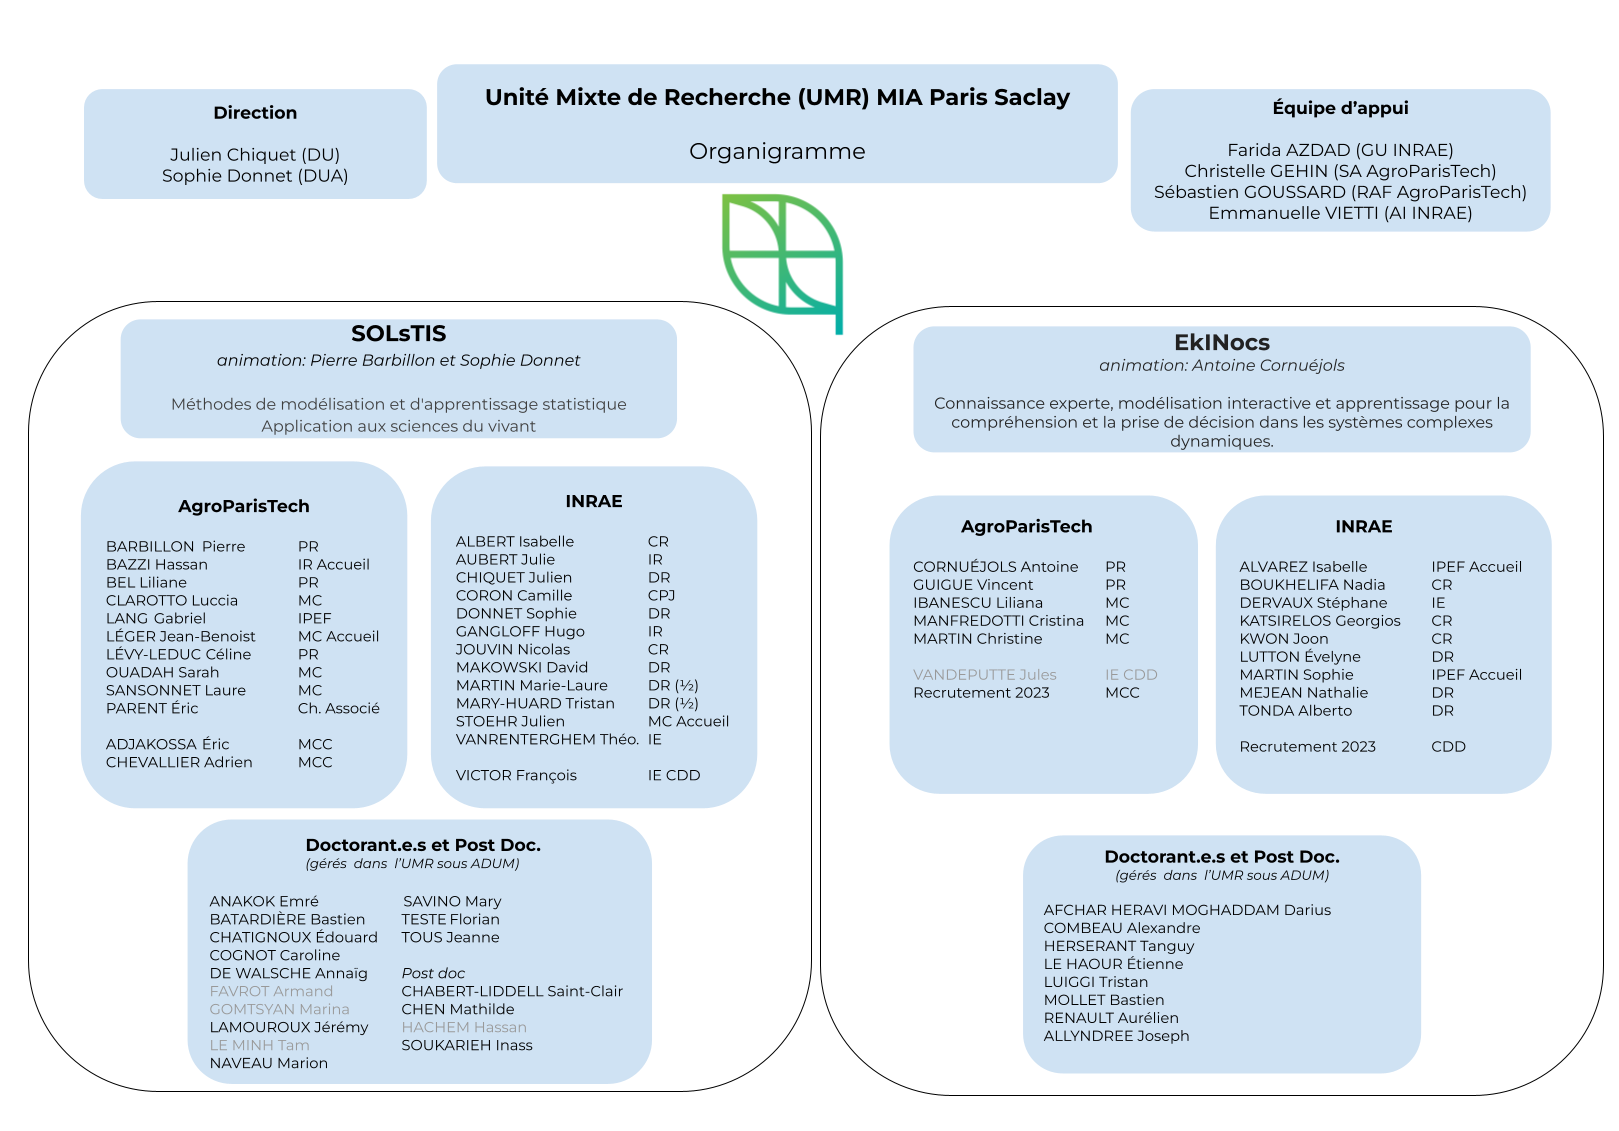
\includegraphics[width=16cm]{organigrammeEquipe.png}
        \caption{Organigramme de l'UMR MIA Paris-Saclay}
        %legende
    \end{center}
\end{figure}

\lipsum[1-2]

\thispagestyle{fancy}

\section{Contexte Scientifique}

\noindent
Ce stage s'inscrit dans un projet de recherche visant à étudier la littérature
scientifique, par des méthodes de web scrapping (sous Python) et de Text Mining
(sous R), afin d'analyser la perception du vers de terre dans la littérature
scientifique.

\lipsum[1-4]

\section{Objectif de mon travail}

\noindent
Ma mission c'est déroulée en deux parties: premièrement, il m'a fallu
construire une base de données d'articles scientifique (au sujet des vers de
terre), en m'appuyant sur le requêtage à des bases de métadonnées sur chaque
article. Les informations ont été récupérées via l'API Crossref.
Ensuite, il me faudra mettre en place des scripts de Text Mining sous R pour
analyser les textes extraits d'Internet.
Au départ, j'avais conçu un script visant à Webscrapper des articles sur la
base PubMed, mais il m'a vite fallu repenser ce script pour interroger une base
de données différente,la base de données PubMed ne correspondant pas aux
besoins de mes encadrants de stage.

\lipsum[1-4]

\thispagestyle{fancy}

\chapter[Ressources]{\label{Second Chapitre}Ressources : pratiques
  professionnelles, environnement informatique, outils informatiques et
  statistiques, données}
\section{Environnement informatique}
\noindent

\section{Pratique Professionnelle}
\noindent
Donec varius orci eget risus. Duis nibh mi, congue eu, accumsan eleifend,
sagittis quis, diam. Duis eget
orci sit amet orci dignissim rutrum

\subsection{Veille bibliographique et technologique}
\noindent
Lorem ipsum dolor sit amet, consectetuer adipiscing elit. Ut purus elit,
vestibulum ut, placerat ac,
adipiscing vitae, felis. Curabitur dictum gravida mauris. Nam arcu libero,
nonummy eget, consectetuer

\subsection[Bonnes pratiques]{Bonne pratique de programmation informatique et
    de developpement logiciel}
\noindent
En concertation avec mes encadrants, j'ai utilisé un dépôt GitHub spécialement
mis en place pour le projet entre eux et moi, où mon travail de chaque jour a
pu être sauvegardé grâce à un mécanisme de Push/Pull. Pour faciliter
l'utilisation de cet outil, le logiciel GitHub Desktop m'a été présenté, une
interface utilisateur graphique facilitant grandement la visualisation et
l'usage du dépôt mis en place pour le projet.

Grâce à la fonctionnalité Knitr de Rmd, j'ai pu rendre compte de ma progression
quotidienne en produisant automatiquement un fichier rapport au format HTML,
directement issue de mon code (figures produites sous R, titres et
intérprétation rédigées en Markdown).

\subsection{Communication des travaux}
\noindent
Lorem ipsum dolor sit amet, consectetuer adipiscing elit. Ut purus elit,
vestibulum ut, placerat ac,
adipiscing vitae, felis. Curabitur dictum gravida mauris. Nam arcu libero,
nonummy eget, consectetuer

\thispagestyle{fancy}

\section[Outils informatiques et statistiques]{Outils informatiques et
  statistiques pour les différentes phases de vos travaux}

\subsection{Récupération des abstracts et métadonnées avec Python}
\noindent
J'ai travaillé sous Python, notamment sous VScode et Spyder (pour le code
Python). J'ai surtout utilisé le package Python Habanero Crossref pour requêter
(en utilisant une API) la base de données Crossref, qui contient une grande
quantité de métadonnées (donnés sur les articles en tant que tel, comme
l'abstract, les auteurs, etc.), afin de récupérer les informations voulue à
propos d'un ensemble de titres d'articles scientifiques défini au préalable sur
le sujet des vers de terre. Pour compléter les données récupérées (la base de
Crossref comprenant de nombreuses données manquantes), j'ai aussi développé en
parallèle un module pour récupérer les données d'intérêt dans le code source de
ResearchGate (web scrapping), comme le \textit{DOI (Digital Object Identifier)}
de chaque publication, la date de chargement sur la base de RG ou encore le
lien vers la page RG correspondante.

\subsection{Text Mining avec R}
\noindent
Pour réaliser le text-mining, j'ai utilisé un script R (développé sous Rstudio
en Rmd) pour traiter le texte et l'analyser sous forme de figures. L'approche
choisie est une approche "tidy" reposant sur la \textit{tokenisation} du corpus
de texte en unitées textuelles (appelées \textit{"tokens"}) plus petite, comme
des mots, des phrases ou des \textit{n-grams}. J'ai pour cela pu m'inspirer du
livre rédigé par Julia Slige (data scientist) et David Robinson (Directeur de
Data Scientist de la plateforme Heap), disponible en ligne à l'adresse:
https://www.tidytextmining.com/. Mon travail a donc consisté à adapter les
codes R montrés en exemple sur des livres à mes propres données (abstracts
d'articles scientifiques), structurées différemment. Les analyses portaient par
exemple sur la fréquence des mots, au global et pour chaque MA, ou encore sur
l'analyse de sentiment (Pour répondre à la question : Quel est le sentiment
global exprimé par le texte à la lecture ?), reposant sur l'attribution d'un
score positif (+1) ou négatif (-1) à chaque mot du corpus. Cette attribution de
sentiment a pu être réalisée grâce à un dictionnaire R conçu pour relier un
token donné à la valence (positive ou négative) qui lui correspond. Afin de
mieux visualiser les résultats, différentes figures ont été réalisées, comme
des diagrammes en barre ou des nuages de mots.

Afin de filtrer les mots d'intérêt seulement, deux stratégies ont été
employées: Premièrement, un filtrage brut de tous les mots de liaisons sans
rapport direct avec le sujet (nommés "stop words" en text-mining, des mots tels
que "the", "and", "is", "of" etc. en anglais) pour ne conserver que les mots
sur lesquels les analyses pourront donner des résultats scientifiques
significatifs (savoir que le mot "le" est le plus fréquent dans un corpus de
texte français ne signifie rien sur le plan biologique). Deuxièmement, une
autre approche a été de considérer la fréquence de chaque mot par rapport au
nombre total de mots présents dans le corpus (n mot / N mots). De cette façon,
on peut visualiser la fréquence des termes sous forme d'histogramme, sans même
avoir besoin de modifier les données au préalable avec une liste de stop words.
Cela permet de conserver le texte dans son ensemble, évitant ainsi un potentiel
biais pouvant perturber l'analyse.

basé sur des méthodes de LDA et de DTM. LDA est une méthode de topic modeling
conçue pour déterminer les thèmes sous-jacents dans un corpus de texte. Les
matrices DTM (Document Term Matrix) sont aussi utilisées pour l'analyse de
texte: ce sont des tableaux en 2 dimensions (les lignes contiennent la liste
des documents / les colonnes représentent les mots-clé) représentant la
fréquence de chaque mot-clé dans chaque document. Grâce à ces méthodes, nous
analyserons le corpus de texte fourni pour étudier la littérature scientifique
sur le sujet des vers de terre. (POUR LA FIN DU STAGE).

\subsection{Ressource 3}
\noindent

\subsection{Ressource 4}
\noindent

\section{Données}
\noindent

\subsection{Données 1}
\noindent
Lorem ipsum dolor sit amet, consectetuer adipiscing elit. Ut purus elit,
vestibulum ut, placerat ac,

\subsection{Données 2}
\noindent
Lorem ipsum dolor sit amet, consectetuer adipiscing elit. Ut purus elit,
vestibulum ut, placerat ac,

\subsection{Données 3}
\noindent
Lorem ipsum dolor sit amet, consectetuer adipiscing elit. Ut purus elit,
vestibulum ut, placerat ac,

\chapter{\label{Troisième Chapitre}Résultats}

\section{Choix et sélection des outils}
\noindent
Pour déveloper mon code de Web scrapping comme ma mission l'exigeait, j'ai
utilisé Python, la langage de scripts avec lequel je suis le plus à l'aise.

\vspace{\baselineskip}

\noindent
\underline{Modules employés pour l'élaboration du code Python:}

\begin{description}
    \item[Pandas:] Pandas est un module qui permet de manipuler facilement des
        tableaux de données avec des étiquettes de variables (colonnes) et d'individus
        (lignes). Il est notamment utilisé dans le script pour exporter les résulats
        issus du code Python vers un fichier CSV(coma separated values), lisible et
        modifiable à l'aide d'outils de bureautique courants comme LibreOffice Calc ou
        Excel.

    \item[Numpy:] Package conçu pour le calcul scientifique avec Python. Il est
        très utile pour l'algèbre (comme par exemple pour la manipulation de matrices),
        et son implémentation en C, C++ et Fortran en fait un outil de calcul rapide et
        efficace pour l'analyse de données et le calcul scientifique. Dans le code,
        cela dit, il sert simplement à l'indexage lors de la création du DataFrame de
        résultats.

    \item[Itertools:] Module implémentant des outils Python pour maîtriser plus
        subtilement les itérations. La méthode employée dans le code est
        \textit{zip\_longest}, qui permet de créer un DataFrame à partir d'une liste de
        listes de tailles potentiellement différentes. La plus longue sera employée en
        référence (longest), et toutes les autres seront ajustées à cette longueur par
        l'ajout d'une \textit{fillvalue} ("null", dans le code). Dans mon travail, elle
        a servi à créer le DataFrame requis à partir de listes de données de tailles
        pas forcément égales (à cause des valeurs manquantes).

    \item[Habanero:] Module client de bas niveau pour interroger l'API
        Crossref, une base de données contenant les métadata des articles de tous les
        membres (des informations comme le titre, le nom d'auteur, le DOI etc.). Dans
        le code Python, elle est employée surtout pour rechercher les noms d'auteurs,
        les autres champs testés n'étant pas assez fiables pour automatiser
        complètement la récupération d'informations. Crossref est codé comme une
        \textbf{classe} du module Habanero, comprenant les méthodes works(), members(),
        prefixes(), funders(), journal(), type() et licence(). Dans le code Python,
        seule la méthode works() a été employée pour envoyer une requête à partir du
        titre de chaque article.

    \item[Unidecode:] Module contenant des fonctions (comme la fonction éponyme
        'unidecode' employée dans le script) conçue pour transformer les chaînes de
        caractères contenant des caractères non-ASCII (comme par exemple des
        idéogrammes chinois) pour les traduire en chaînes de caractères contenant
        uniquement des caractères ASCII. Dans le code, la méthode \textit{unidecode}
        est employée pour rendre l'affichage des noms d'auteur contenant des caractères
        non-ASCII. Certaines corrections sont imparfaites et retirent quelques lettres.

    \item[RGS2:] Sous-module codé localement à partir d'un exemple trouvé en
        ligne\footnote{\url{https://www.reddit.com/r/Python/comments/v2bxyl/script_scraping_researchgate_all_publications/}}
        , par la suite adapté pour récupérer directement les informations
        voulues dans le code source du site scientifique ResearchGate, les autres
        options potentielles (comme Google Scholar) ayant souvent un système de
        détection et de blocage des bots. Seule la deuxième version du sous-module a
        été retenue dans le projet final. Il dépend des modules suivants :
        \begin{enumerate}
            \item Module \textbf{Parsel}, fonction \textit{Selector}: Module
                  facilitant l'extraction des données pour les formats HTML, JSON et XML. Dans le
                  code, il est utilisé pour trouver les données recherchées directement dans le
                  code source de la page (web scrapping) en s'appuyant sur des sélecteurs CSS.
                  \vspace{\baselineskip}
            \item Module \textbf{playwright.sync\_api}, fonction
                  \textit{sync\_playwright}: Module permettant de lancer une session navigateur
                  depuis un script Python. Dans le code, il est utilisé pour se rendre sur le
                  site de ResearchGate via une session Chromium, un navigateur libre développé
                  par Google.
                  \vspace{\baselineskip}
            \item Module \textbf{re}: Module fournissant des opérations sur les
                  expressions rationnelles utilisable dans un code Python, ce qui peut s'avérer
                  nécessaire pour sélectionner très précisément les informations voulues dans une
                  structure de données complexes. Dans le code Python, il est utilisé pour
                  filtrer les résultats HTML bruts issus du Web scrapping.
                  \vspace{\baselineskip}
            \item Module \textbf{time}, fonction \textit{sleep}: Module
                  fournissant différentes fonctions liées au temps. Dans le script, la fonction
                  "sleep(t)" est utilisée pour forcer le système à ne rien faire pendant t
                  secondes, évitant de cette façon de surcharcher le serveur cible de requêtes
                  trop rapides et trop nombreuses.
        \end{enumerate}

        \vspace{\baselineskip}
        \noindent
        Dans un deuxième temps, pour déveloper mon code de text mining comme ma
        mission l'exigeait, j'ai utilisé R, la langage informatique utilisé dans le
        livre qui m'a été fourni en exemple.

        \vspace{\baselineskip}
        \noindent
        \underline{Modules employés pour l'élaboration du code R:}

\end{description}
\noindent

\section{Installation et test des outils}

\section{Conception de la méthode}

\section{Développement de la méthode}

\section{Validation de la méthode}

\section{Résultats biologiques}

\thispagestyle{fancy}

\chapter{\label{Quatrième Chapitre}Discussion}
%\paragraph{Paragraphe}
\noindent
Au cours de ce stage, j'ai commencé par développer un programme Python pour le
web scrapping sur la base de données médicale PubMed, avant de découvrir que ce
n'était pas selon dont nous avions besoin. J'ai donc réussi à m'adapter pour
faire fonctionner mon code (en interrogeant une autre base de données), mais il
reste encore à nettoyer les données extraites par le code (collectées
directement en brut dans un fichier CSV généré par le script).
Rétrospectivement, je ne suis pas certain que cette approche automatisée soit
vraiment rentable en temps, même si je suis satisfait d'avoir commencé à
apprendre comment développer ce type d'approches automatisées.

\lipsum[1]

\thispagestyle{fancy}

\chapter{\label{Cinquième Chapitre}Conclusion}
Elle vise, à reformuler les objectifs visés, énoncer les résultats essentiels
obtenus, à replacer le
travail dans son contexte scientifique et à faire ressortir leur importance
théorique, pratique, tech-
nique ou économique. Elle peut ouvrir de nouvelles perspectives ou hypothèses
qui seront le point
de départ de nouveaux travaux. Il n'y a pas a priori d'appel à des références.

\thispagestyle{fancy}

%%%%%%%%%%%%%%%%%%%%%%%%%%%%%%%%%%%%%%%%          15         %%%%%%%%%%%%%%%%%%%%%%%%%%%%%%%%%%%%%%%%%%%%%%%%%%%%%%%%%%%%%%%%%%%%%%%%%%%%%%%%%%%%%%%%%% Références %%%%%%%%%%%%%%%%%%%%%%%%%%%%%%%%%%%%%%%%%%%%%%%%
\newpage
\bibliographystyle{plain}
\bibliography{mabiblio}
\cite{clef1}
\thispagestyle{fancy}
%\apalike

%%%%%%%%%%%%%%%%%%%%%%%%%%%%%%%%%%%%%%%%          16            %%%%%%%%%%%%%%%%%%%%%%%%%%%%%%%%%%%%%%%%%%%%%%%%%%%%%%%%%%%%%%%%%%%%%%%%%%%%%%%%%%%%%%%%%% Verso Résumé %%%%%%%%%%%%%%%%%%%%%%%%%%%%%%%%%%%%%%%%%%%%%%%%

\newpage
\thispagestyle{empty}
\mbox{} % Insère une boîte vide

%%%%%%%%%%%%%%%%%%%%%%%%%%%%%%%%%%%%%%%%          17            %%%%%%%%%%%%%%%%%%%%%%%%%%%%%%%%%%%%%%%%%%%%%%%%%%%%%%%%%%%%%%%%%%%%%%%%%%%%%%%%%%%%%%%%%% Résumé %%%%%%%%%%%%%%%%%%%%%%%%%%%%%%%%%%%%%%%%%%%%%%%%

\newpage
\thispagestyle{empty}
\begin{center}
    \huge{\textbf{Résumé}}
\end{center}

\vspace{1cm}
En résumé, ce stage m’a permis d'apprendre les bases du web scrapping
automatisé avec Python (pour la veille bibliographique) et du Text Mining avec
R pour chercher automatiquement des mots clés d'intérêt dans la littérature.
Cela m'a également permis de prendre conscience que même au sein de la
communauté scientifique, la perception d'un même sujet (ici, le vers de terre),
peut-être totalement différente, voire opposée, d'un pays à l'autres.

\vspace{\baselineskip} % Sauter une ligne
\par
\textbf{Mots-clés de référencement type MESH :}
\vspace{\baselineskip} % Sauter une ligne
\par
\textbf{Mots-clés des acquis techniques : }

\end{document}

%\it = italique
% \sl = mettre en travers
% {\bf texte}
%\textbf{texte}
%vfill
%hspace{2cm} va mettre un espace entre les logos
% \thispagestyle{empty}
% renewcommand{\thechapter{Roman}} = redefinir la maniere dont la numerotation se fait pour les chaptire :refaire la commande en chiffre romain
% renewcommand{\thechapter{roman}} = chiffres romains en minuscules
% renewcommand{\thechapter{Arabic}}
%\arabic % à mettre avant le begin du doc
%\alph
%créer une nouvelle commande : \newcommand{\convertToBW}[1]{\adjustimage{filter=gray}{#1}}
%le _ permet de mettre en indice. Il peut facilement tout bousiller si mal utilisé.
% (\href{https://www.reddit.com/r/Python/comments/v2bxyl/script_scraping_researchgate_all_publications/}{\texttt{https://www.redd\linebreak it.com/r/Python/comments/v2bxyl/script\_scraping\_researchgate\_all\_publica\linebreak tions/}})